\documentclass[compress]{beamer}

\usepackage[utf8]{inputenc}
\usepackage{graphicx}
\usepackage{varwidth}
\usepackage{beamerthemesplit} 

\usepackage[english]{babel}
\usepackage[backend=bibtex]{biblatex}
\addbibresource{bibliography.bib}

\useoutertheme{miniframes}


\usetheme[progressbar=frametitle]{Madrid}
\usefonttheme{professionalfonts}
\setbeamertemplate{itemize items}[triangle]
\setbeamertemplate{enumerate items}[default]
\usecolortheme{beaver}

%Information to be included in the title page:

\title[COVID-19 - Unsupervised Learning]{A statistical analysis on factors that contributed/slowed down the spread of COVID-19}

\author{Marzio De Corato}

\subtitle{Project for the exam: Machine learning, statistical
learning, deep learning and artificial intelligence - Unsupervised Learning}

\begin{document}

\frame{\titlepage}

\section{Intro}

\begin{frame}
\frametitle{Overview}
\textbf{FINAL GOAL}: Survey the statistical correlations between the COVID-19 cases/deaths and a selected set of attributes for different clusters via the principal component analysis 
\newline
\newline
\textbf{CLUSTERS}: Provinces (IT), Regions (IT), Countries

\end{frame}

\section{Data}

\begin{frame}
\frametitle{Cluster features}
\begin{columns}
\column{0.3\textwidth}
\textbf{Provices (IT)}
\begin{itemize}
\item Unemployment '19
\item Private Transport '12 
\item Air Quality '19
\item Public Transport '12
\item Density '19
\item Mean income '19
\end{itemize}
\column{0.3\textwidth}
\textbf{Regions (IT)}
\begin{itemize}
\item Mortality
\item Pop. for GP
\item Mean Income '19
\item Number of Visits for Pop. '17
\item Public Transport 
\item Density '19
\item Mean income '19
\item Tests 
\item LEA '17
\item Number of visit '17
\item Public structures '17
\end{itemize}
\column{0.3\textwidth}
\textbf{Countries}
\begin{itemize}
\item PM$_{2.5}$ '16
\item Traffic Mortality '16
\item Pollution Mortality '16
\item GDP pro-capita '19
\item Health expenditure '17
\item UHC '17
\end{itemize}
\end{columns}
\end{frame}

\begin{frame}
\frametitle{Datasets features }

\textbf{TEMPORAL INTERVAL}: Provinces up to 24/08/2020; Regions up to 24/08/2020; Countries up to 27/08/2020 
\newline
\newline
\textbf{SOURCES}: Protezione Civile, Istituto Italiano di Statistica, Ministro delle Finanze, Ministro della Salute, World Health Organization and World Bank 

\end{frame}

\begin{frame}
\frametitle{Provinces}

\begin{figure}[H]
\centering
\begin{minipage}{.6\textwidth}
  \centering
  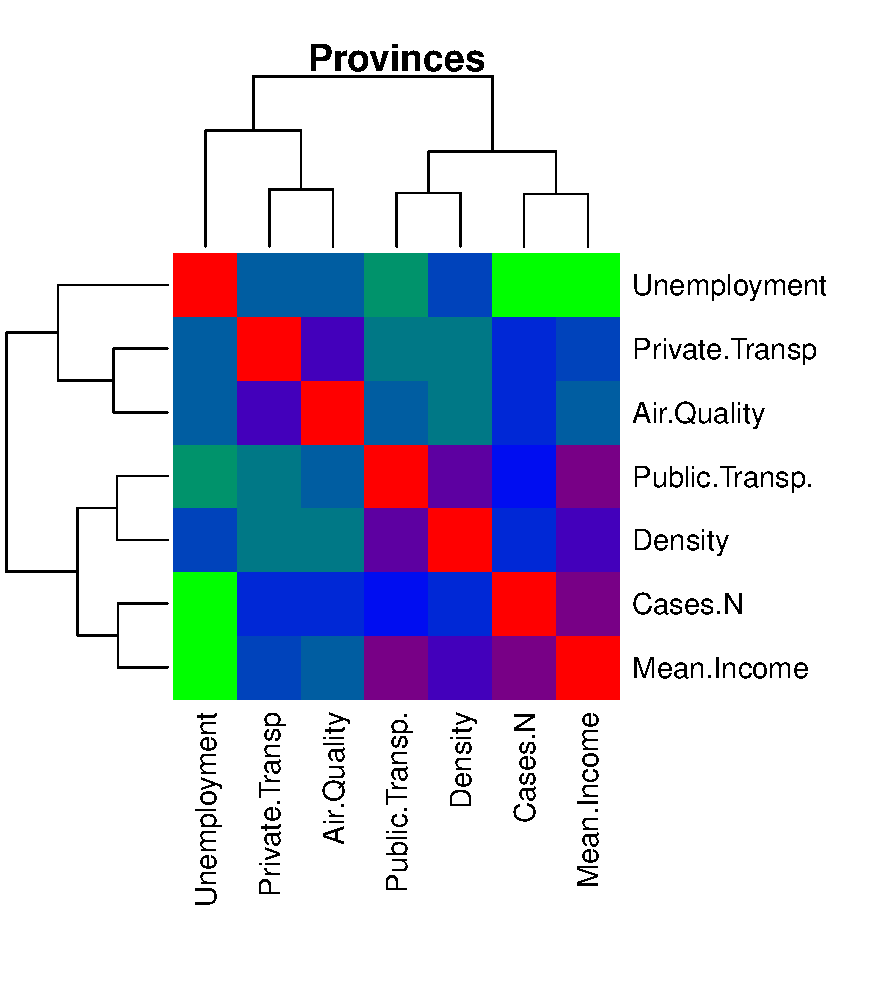
\includegraphics[width=\linewidth, ]{Pic/Province_FULL_CorrMatrix.pdf}
\end{minipage}%
\begin{minipage}{.3\textwidth}
  \centering
  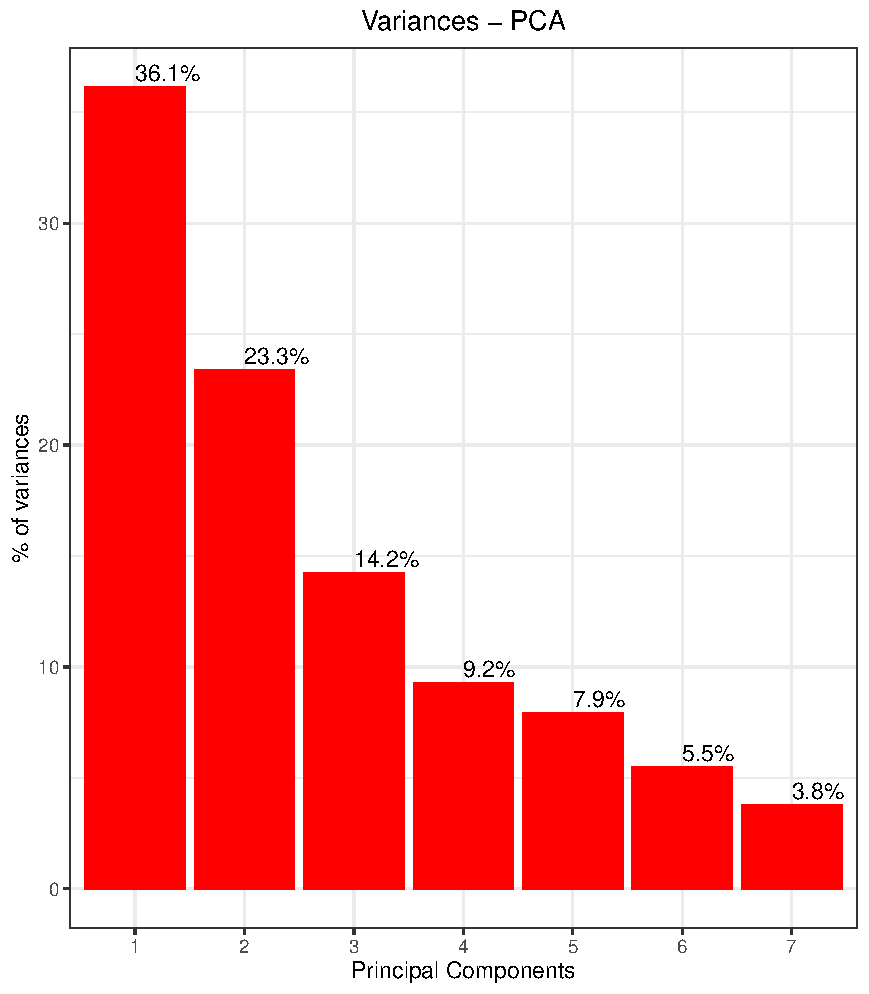
\includegraphics[width=\linewidth,]{Pic/Province_FULL_Variances.pdf}
\end{minipage}
\end{figure}
\end{frame}

\begin{frame}


\frametitle{Provinces}


\begin{figure}[H]
\centering
\begin{minipage}{.5\textwidth}
  \centering
  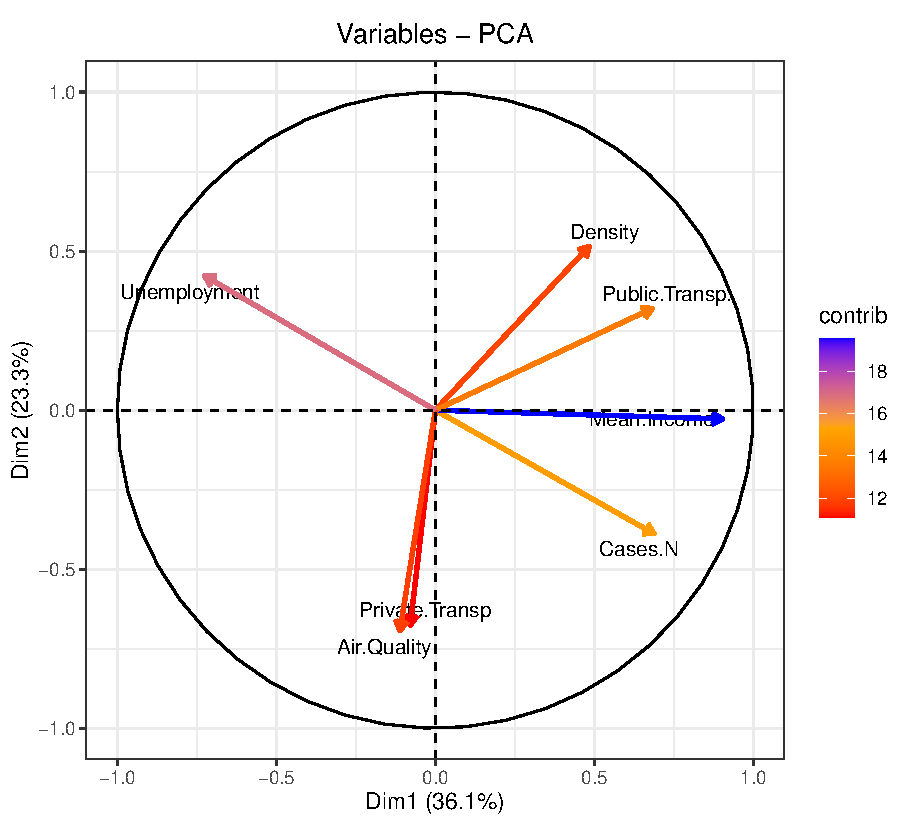
\includegraphics[width=\linewidth, ]{Pic/Province_FULL_Variables-PCA.pdf}
\end{minipage}%
\begin{minipage}{.5\textwidth}
  \centering
  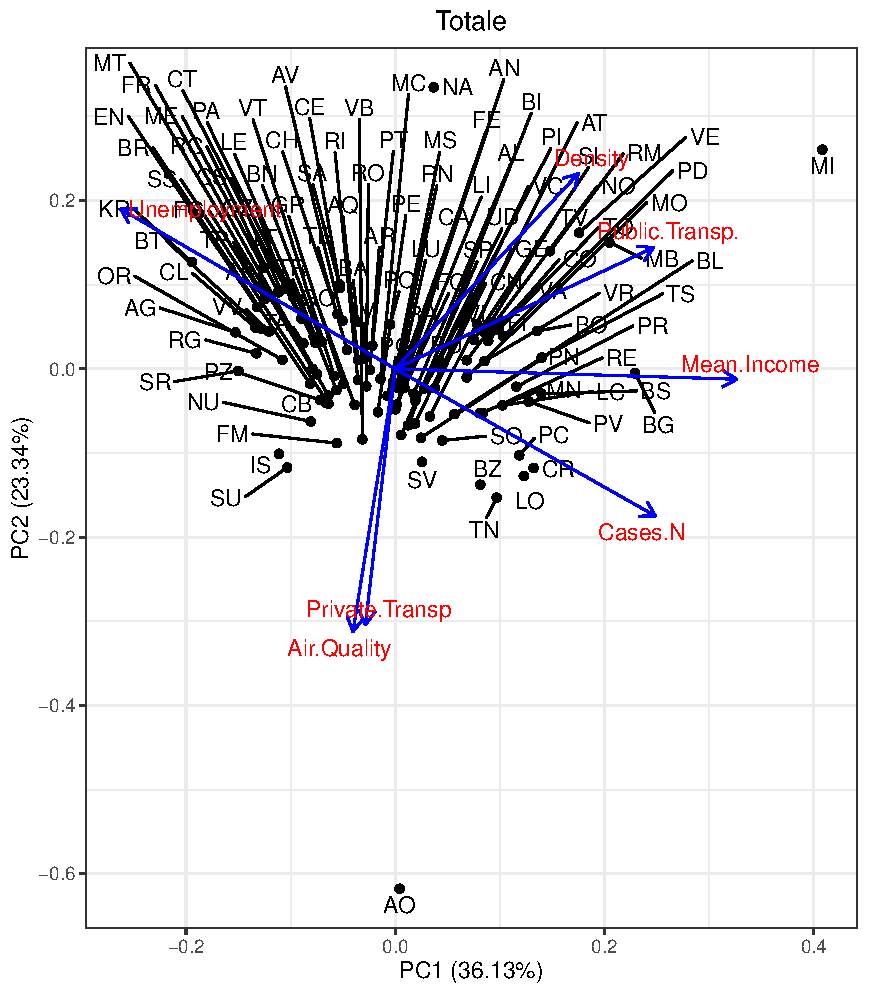
\includegraphics[width=\linewidth,]{Pic/Provinces_PCA_FULL.pdf}
\end{minipage}
\end{figure}

\end{frame}

\begin{frame}


\frametitle{Provinces - Conclusions}

\begin{columns}
\column{0.5\textwidth}
\begin{figure}[H]
\centering
\begin{minipage}{\textwidth}
  \centering
  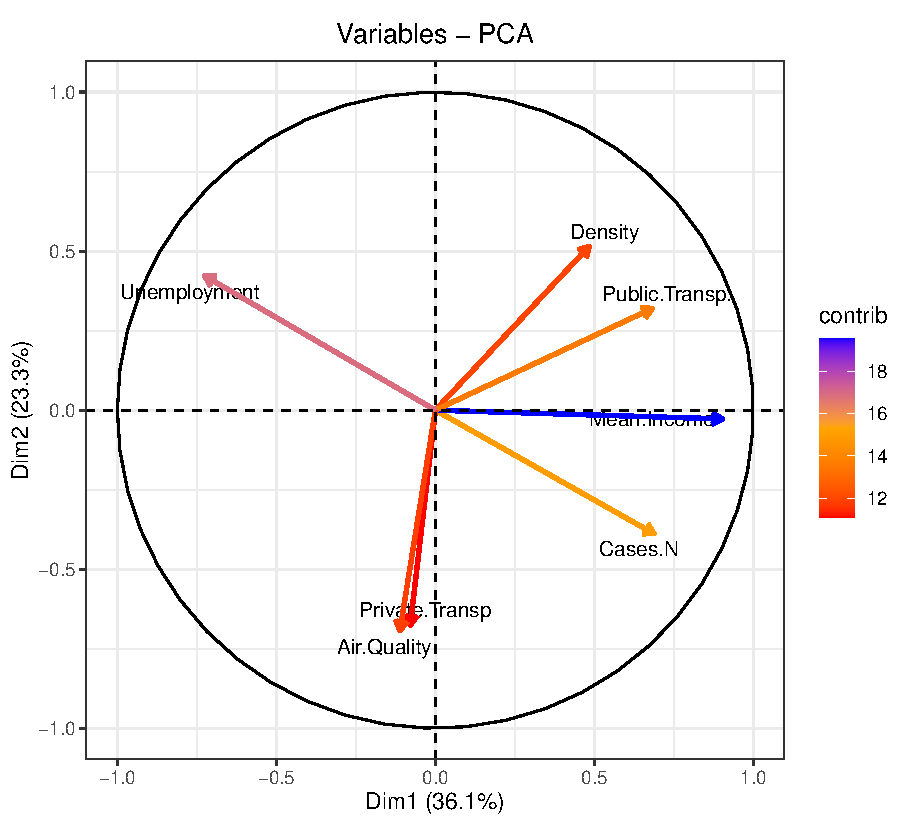
\includegraphics[width=\linewidth, ]{Pic/Province_FULL_Variables-PCA.pdf}
\end{minipage}%
\end{figure}
\column{0.5\textwidth}
\begin{itemize}
\item The public transport, the density, the normalized cumulative cases and the mean income are positively correlated
\item A higher density, a higher public transport demand and a higher income increase the rate of contact between the individuals \cite{neiderud2015urbanization,world2010hidden}
\item Rich people can spend more money for social events or perhaps in to travels thus they increase their connectivity (the opposite happens for the unemployment)\cite{weyers2008low}
\end{itemize}
\end{columns}
\end{frame}



\begin{frame}
\frametitle{Regions}

\begin{figure}[H]
\centering
\begin{minipage}{.6\textwidth}
  \centering
  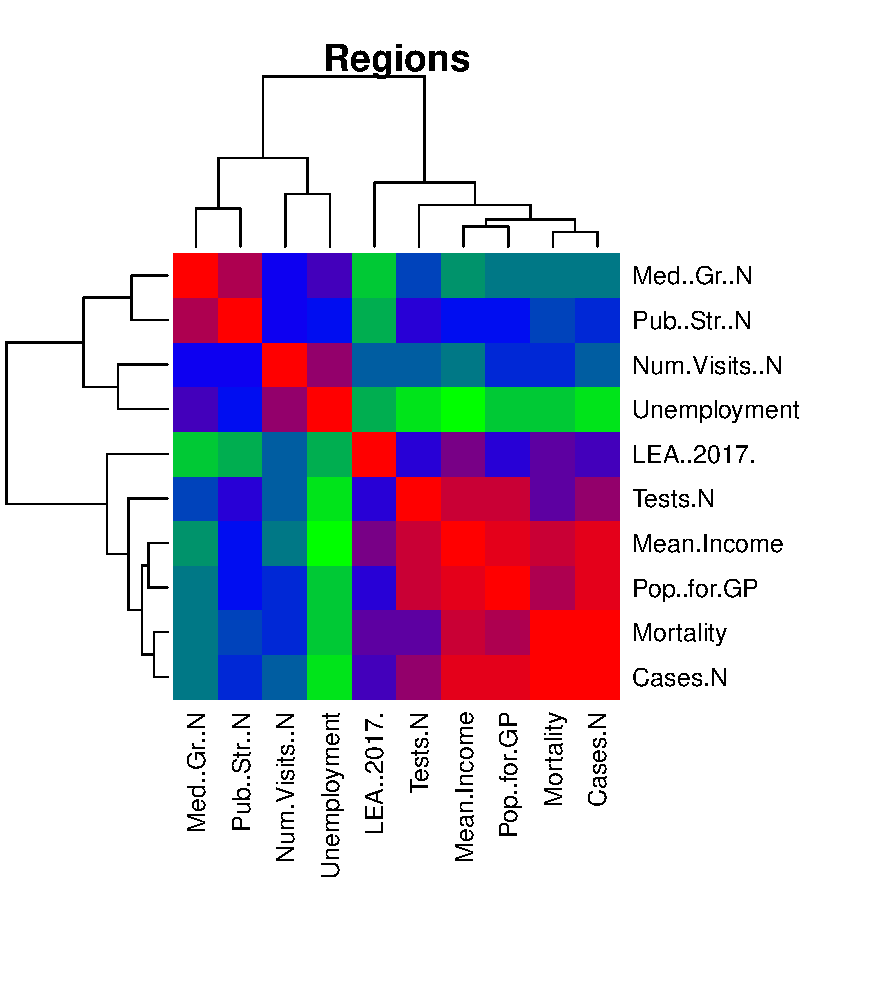
\includegraphics[width=\linewidth, ]{Pic/Regions_CorrMatrix.pdf}
\end{minipage}%
\begin{minipage}{.3\textwidth}
  \centering
  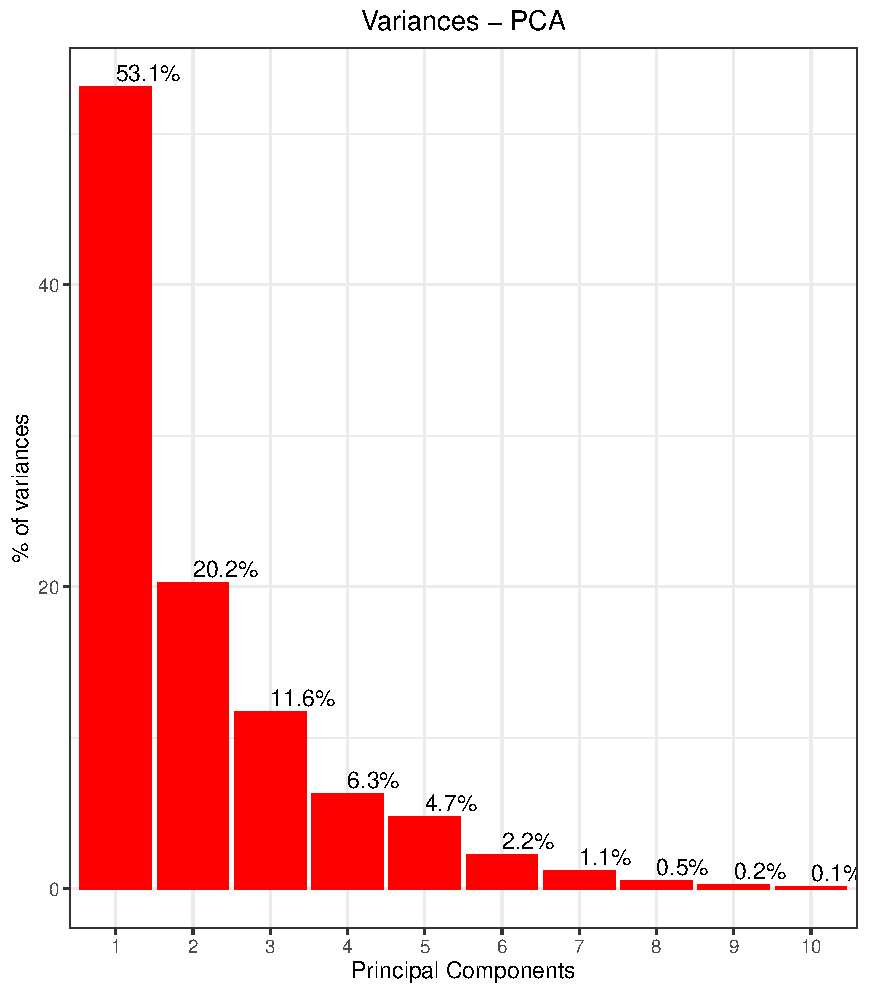
\includegraphics[width=\linewidth,]{Pic/Region_variances.pdf}
\end{minipage}
\end{figure}
\end{frame}

\begin{frame}
\frametitle{Regions}

\begin{figure}[H]
\centering
\begin{minipage}{.5\textwidth}
  \centering
  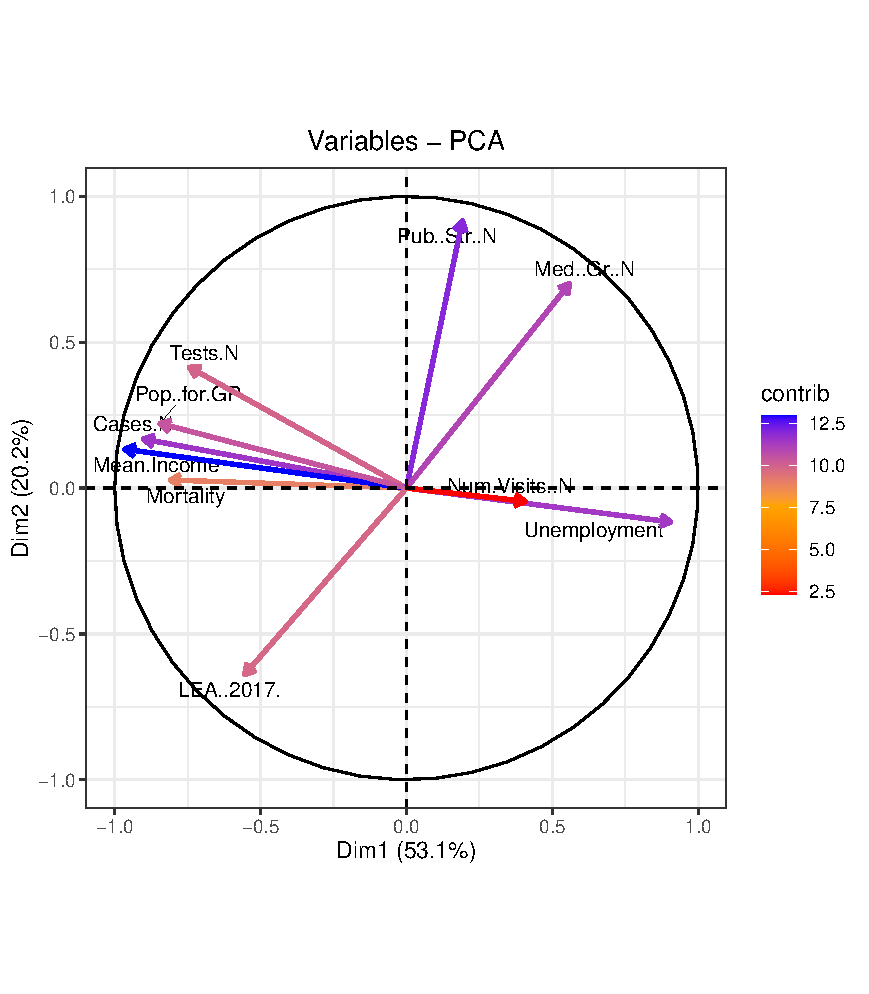
\includegraphics[width=\linewidth, ]{Pic/Regioni_PCA_loadings.pdf}
\end{minipage}%
\begin{minipage}{.5\textwidth}
  \centering
  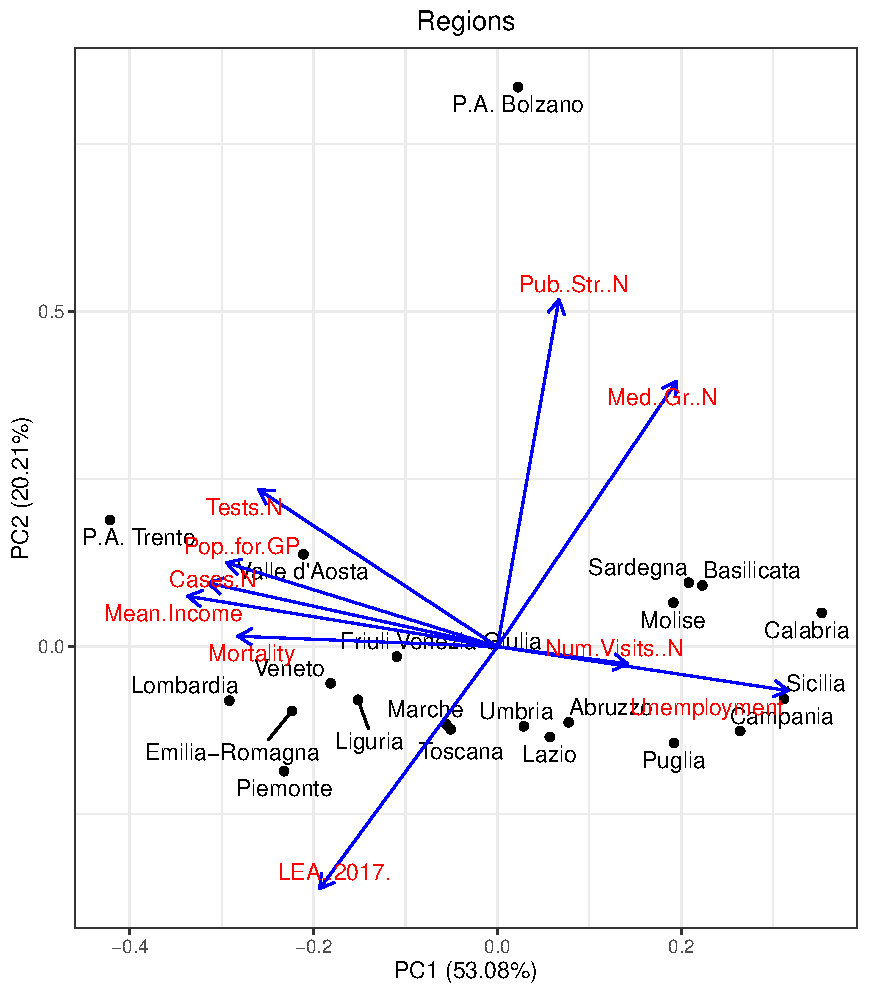
\includegraphics[width=\linewidth,]{Pic/Regions_FULL_PCA.pdf}
\end{minipage}
\end{figure}
\end{frame}


\begin{frame}
\frametitle{Regions - Conclusions}
\begin{columns}
\column{0.5\textwidth}
\begin{figure}[H]
\centering
\begin{minipage}{\textwidth}
  \centering
  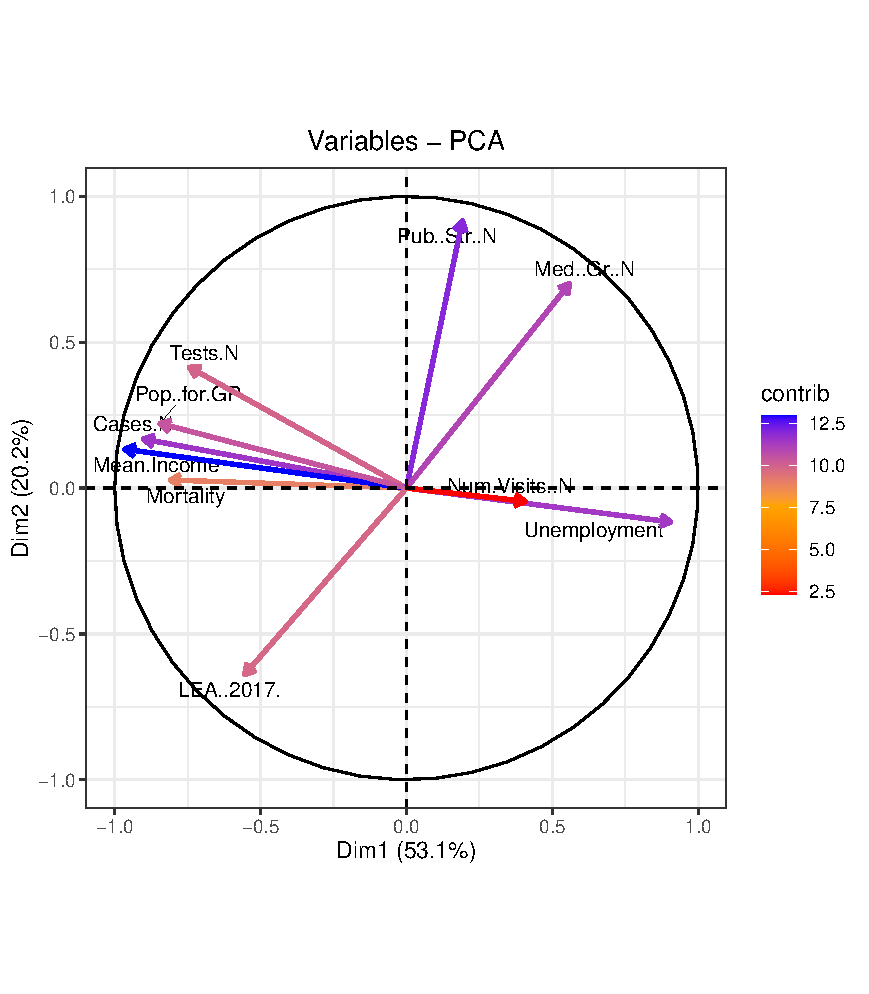
\includegraphics[width=\linewidth, ]{Pic/Regioni_PCA_loadings.pdf}
\end{minipage}%
\end{figure}
\column{0.5\textwidth}
\begin{itemize}
\item Positive correlation between the number of people for general practitioner(GP) and the number of cases
\item A higher number of normalized visit is negatively correlated with the number of cases and the mortality
\item The GP play the role of sensor for the COVID-19 cases:if their number and their presence is reduced, the health service is less sensitive to find new cases and the diffusion of the virus is favoured \cite{24plus}

\end{itemize}
\end{columns}
\end{frame}


\begin{frame}
\frametitle{Countries}
\begin{figure}[H]
\centering
\begin{minipage}{.6\textwidth}
  \centering
  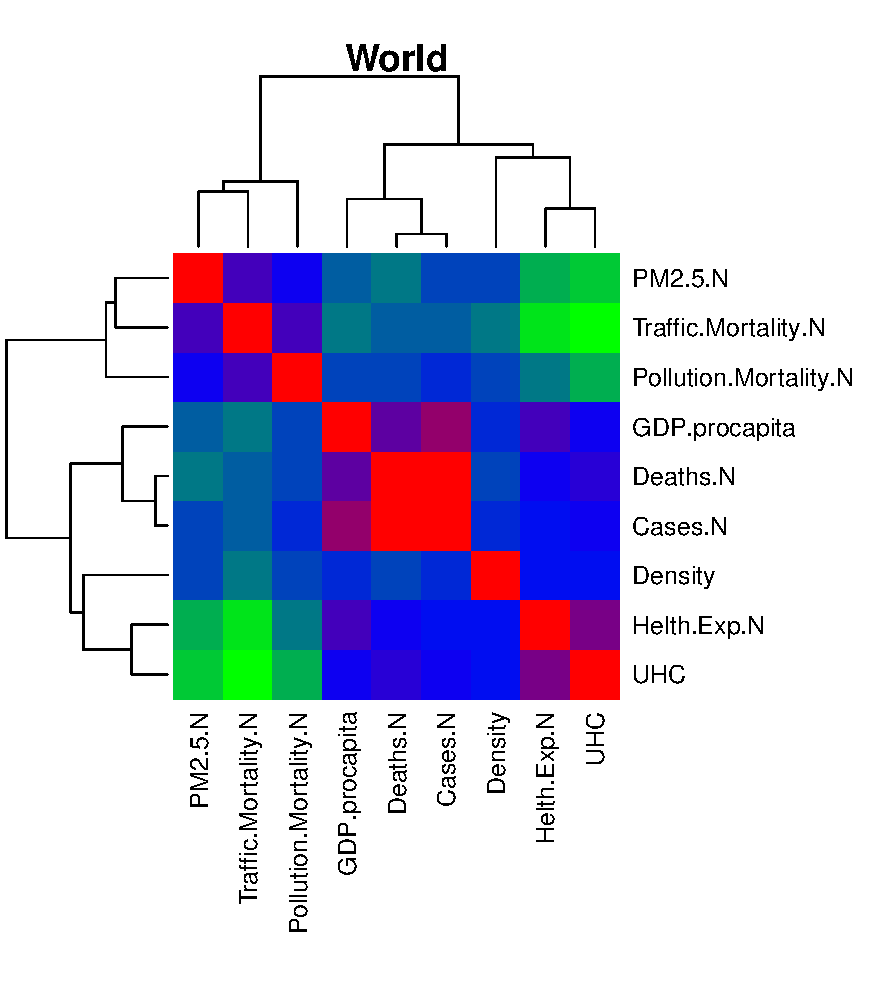
\includegraphics[width=\linewidth, ]{Pic/CorrMatrix_WORLD.pdf}
\end{minipage}%
\begin{minipage}{.3\textwidth}
  \centering
  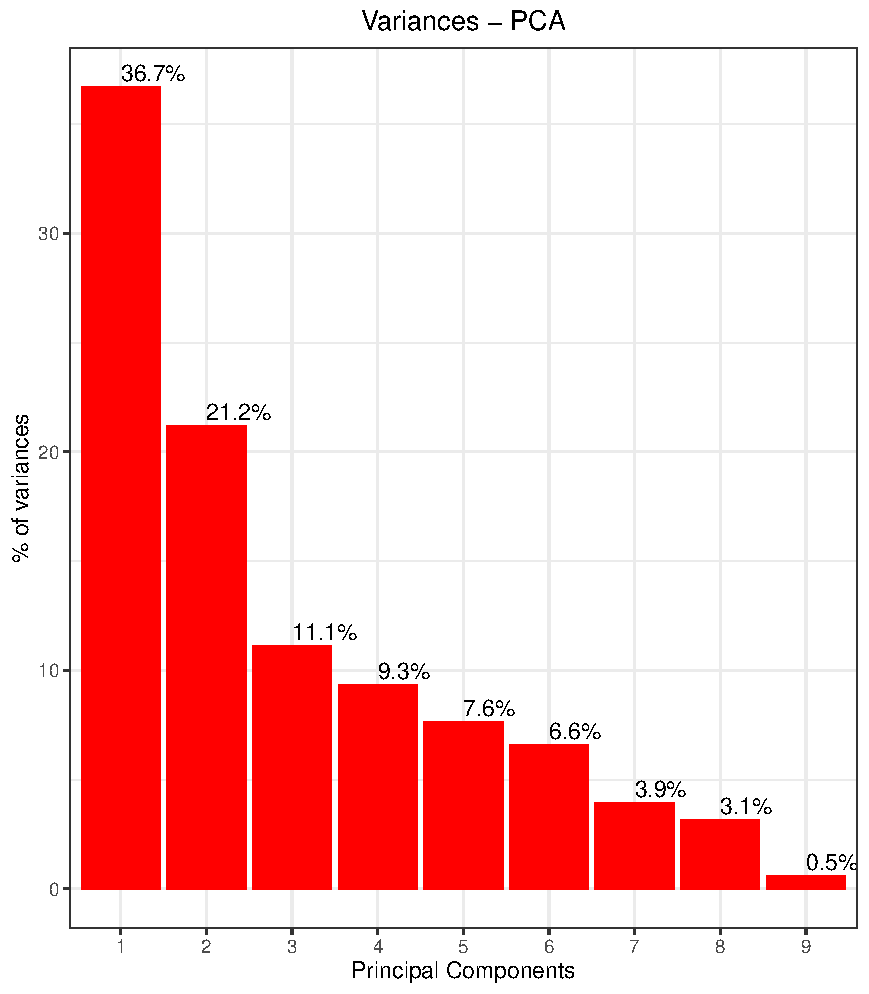
\includegraphics[width=\linewidth,]{Pic/Variances-PCA_WORLD.pdf}
\end{minipage}
\end{figure}
\end{frame}

\begin{frame}
\frametitle{Countries}
\begin{figure}[H]
\centering
\begin{minipage}{.5\textwidth}
  \centering
  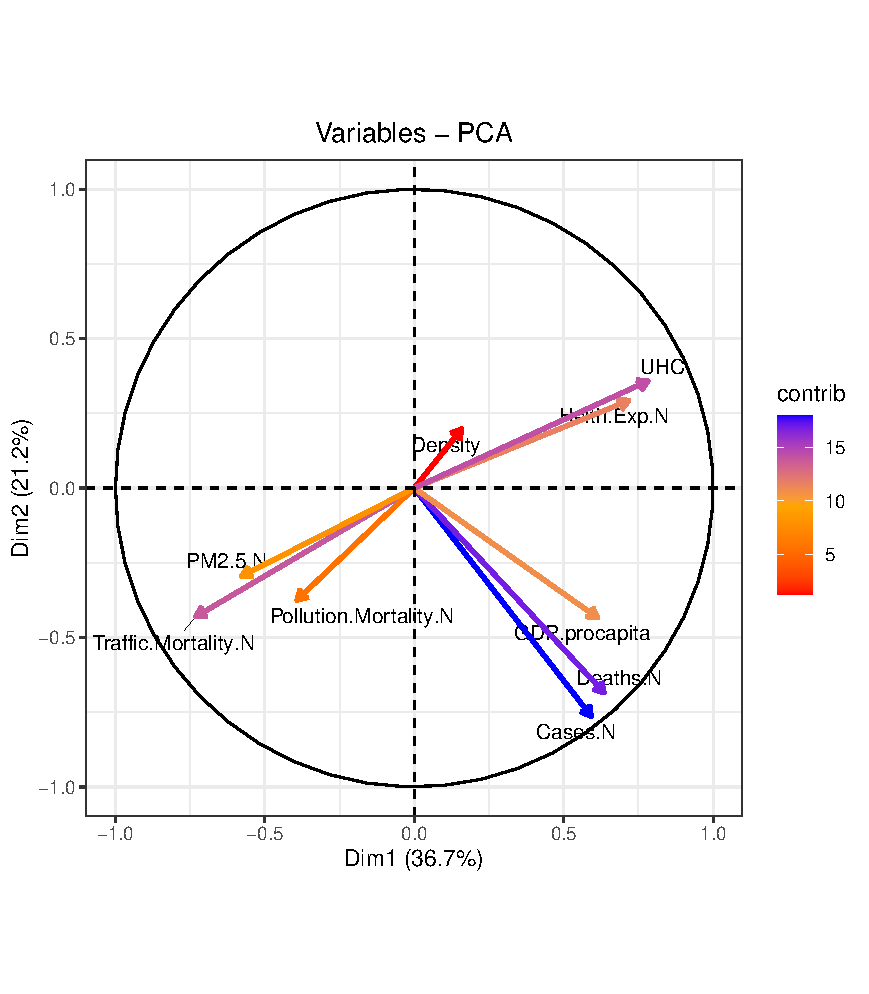
\includegraphics[width=\linewidth, ]{Pic/PCA-Loadings_WORLD.pdf}
\end{minipage}%
\begin{minipage}{.5\textwidth}
  \centering
  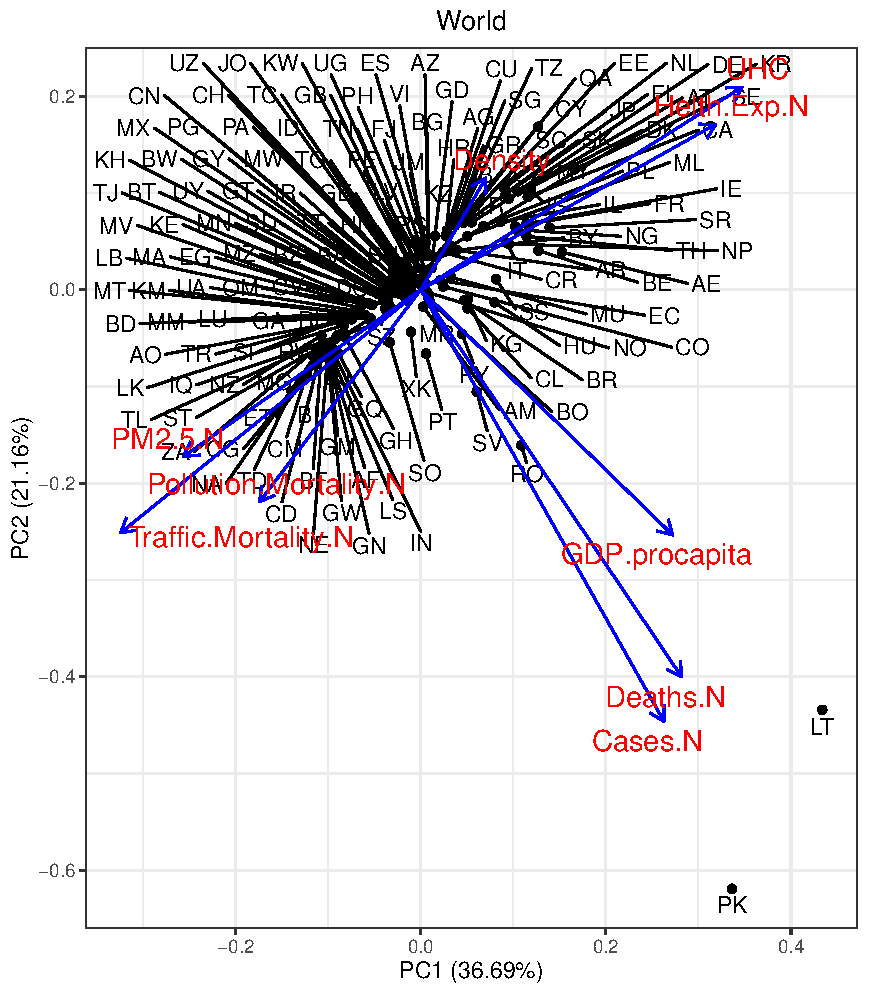
\includegraphics[width=\linewidth,]{Pic/World_FULLPCA.pdf}
\end{minipage}
\end{figure}
\end{frame}

\begin{frame}
\frametitle{Countries - Conclusions}
\begin{columns}
\column{0.5\textwidth}
\begin{figure}[H]
\centering
\begin{minipage}{\textwidth}
  \centering
  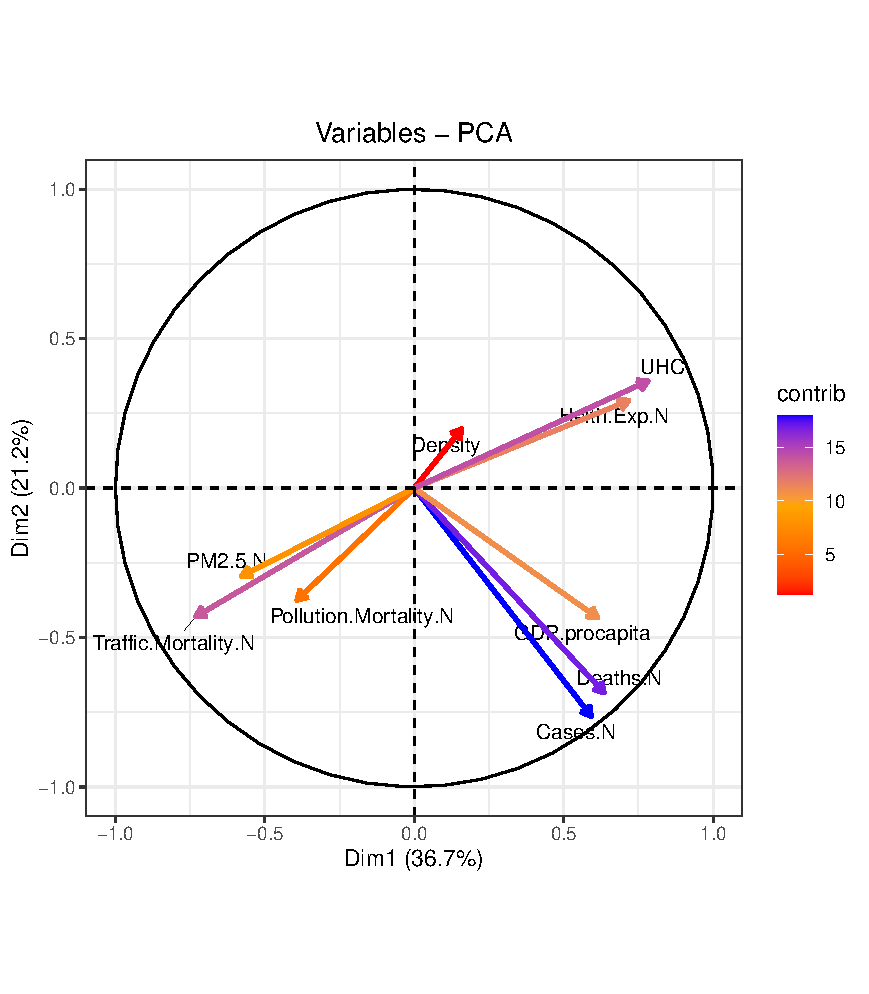
\includegraphics[width=\linewidth, ]{Pic/PCA-Loadings_WORLD.pdf}
\end{minipage}%
\end{figure}
\column{0.5\textwidth}
\begin{itemize}
\item The GDP pro-capita seems to be statistically correlated with the cases and the deaths
\item A possible objection to this link can be that only the richest countries can invest money
for the tests for the validation of a COVID19 case: however it can be noted from plots that the normalized health expenditure as well the UHC index are basically orthogonal with respect to the normalized COVID19 cases and deaths
\end{itemize}
\end{columns}
\end{frame}





\begin{frame}[t,allowframebreaks]
\frametitle{References}
\printbibliography
\end{frame}

\end{document}